% ============================================================
%  FCHEV Graduation Project Defense — Beamer Presentation
%  MAT 4901E  |  Ahmet Yeşil  |  June 2026
%  Compile with:  pdflatex -shell-escape presentation.tex  (×2)
% ============================================================
\documentclass[aspectratio=169, 10pt]{beamer}

% ---------- Theme & Colours ----------
\usetheme{Madrid}
\usecolortheme{whale}
\useinnertheme{circles}

\definecolor{fcblue}{RGB}{0,62,126}
\definecolor{fcgold}{RGB}{255,193,7}
\definecolor{fcgray}{RGB}{96,96,96}

\setbeamercolor{palette primary}{bg=fcblue,fg=white}
\setbeamercolor{palette secondary}{bg=fcblue!80,fg=white}
\setbeamercolor{palette tertiary}{bg=fcblue!60,fg=white}
\setbeamercolor{frametitle}{bg=fcblue,fg=white}
\setbeamercolor{title}{bg=fcblue,fg=white}
\setbeamercolor{block title}{bg=fcblue,fg=white}
\setbeamercolor{alerted text}{fg=fcgold!80!black}
\setbeamercolor{structure}{fg=fcblue}

% ---------- Packages ----------
\usepackage{amsmath,amssymb,bm}
\usepackage{booktabs}
\usepackage{array}
\usepackage{graphicx}
\usepackage{xcolor}
\usepackage{tikz}
\usepackage{pgfplots}
\pgfplotsset{compat=1.18}
\usepackage{fontawesome5}
\usepackage{hyperref}
\usepackage{caption}
\captionsetup{font=scriptsize,labelfont=scriptsize}

% ---------- Speaker Notes ----------
\usepackage{pgfpages}
% Uncomment the next line to show notes on second screen:
% \setbeameroption{show notes on second screen=right}

% ---------- Metadata ----------
\title[FCHEV Energy Management]{Mathematical Modeling \& Control Strategies\\for Hybrid Hydrogen Systems}
\subtitle{MAT 4901E — Graduation Project I Defense}
\author[A.~Yeşil]{\textbf{Ahmet Yeşil} \\ \small Student No: 090220359}
\institute[ITU]{\small Supervisor: \textbf{Prof.\ Dr.\ Semra Ahmetolan} \\[4pt]
Istanbul Technical University — Mathematical Engineering}
\date{June 14, 2026}

% ---------- Custom commands ----------
\newcommand{\PFC}{P_{\mathrm{FC}}}
\newcommand{\Pbat}{P_{\mathrm{bat}}}
\newcommand{\Pload}{P_{\mathrm{load}}}
\newcommand{\SoC}{\mathrm{SoC}}
\newcommand{\etaFC}{\eta_{\mathrm{FC}}}
\newcommand{\MH}{M_{\mathrm{H_2}}}
\newcommand{\Mel}{M_{\mathrm{elec}}}
\newcommand{\LHV}{\mathrm{LHV}_{\mathrm{H_2}}}
\newcommand{\highlight}[1]{\textcolor{fcgold!80!black}{\textbf{#1}}}

% ============================================================
\begin{document}

% ============================================================
%  SLIDE 1 — TITLE
% ============================================================
\begin{frame}[plain]
  \titlepage
\end{frame}
\note{
  Welcome everyone. My name is Ahmet Yeşil and today I will be presenting my graduation project
  titled \textit{Mathematical Modeling and Control Strategies for Hybrid Hydrogen Systems}.
  This work was carried out under the supervision of Prof.\ Dr.\ Semra Ahmetolan as part of
  MAT 4901E. \\[4pt]
  In the next 20–25 minutes I will walk you through why we need a hybrid hydrogen vehicle,
  how we modeled every component mathematically, how we formulated the energy management
  problem, and what we plan to achieve in the second semester.
}

% ============================================================
%  SLIDE 2 — OUTLINE
% ============================================================
\begin{frame}{Outline}
  \tableofcontents[hideallsubsections]
\end{frame}

\section{Motivation \& Problem Definition}
\section{System Architecture}
\section{Mathematical Modeling}
\section{Power Flow \& Cost Function}
\section{Control Strategies}
\section{Future Work}

% ============================================================
%  SLIDE 3 — WHY FCHEV?
% ============================================================
\begin{frame}{Motivation: Why a Fuel Cell Hybrid Vehicle?}
  \begin{columns}[T]
    \begin{column}{0.55\textwidth}
      \begin{block}{The Promise of Hydrogen Mobility}
        \begin{itemize}
          \item \textbf{Zero tailpipe emissions} — only exhaust product is \highlight{water}
          \item High energy density: $\LHV = 120\;\text{MJ/kg}$, vs.\ $\approx 45\;\text{MJ/kg}$ for petrol
          \item Fast refueling ($\sim$3–5 min at 700 bar)
          \item Proton Exchange Membrane Fuel Cell (\textbf{PEMFC}) is the established automotive choice
        \end{itemize}
      \end{block}
      \vspace{4pt}
      \begin{alertblock}{The Core Problem}
        A \textbf{stand-alone} fuel cell cannot meet the demands of daily driving:
        \begin{enumerate}
          \item \highlight{Slow dynamic response} to sudden acceleration
          \item \highlight{Cannot absorb} regenerative braking energy
          \item Frequent load cycling $\Rightarrow$ membrane degradation
        \end{enumerate}
      \end{alertblock}
    \end{column}
    \begin{column}{0.42\textwidth}
      \begin{block}{The Solution: Hybridization}
        \centering
        \begin{tikzpicture}[scale=0.85, every node/.style={font=\small}]
          % FC
          \draw[fill=fcblue!20, rounded corners] (0,2.4) rectangle (2.2,3.4)
            node[midway, align=center] {\faIcon{bolt}\\PEMFC};
          % Battery
          \draw[fill=green!20, rounded corners] (0,0.8) rectangle (2.2,1.8)
            node[midway, align=center] {\faIcon{battery-three-quarters}\\LiFePO$_4$\\Battery};
          % DC Bus
          \draw[fill=fcgold!30, rounded corners] (3.0,1.4) rectangle (4.6,2.4)
            node[midway, align=center] {DC\\Bus};
          % Motor
          \draw[fill=gray!20, rounded corners] (5.4,1.4) rectangle (6.8,2.4)
            node[midway, align=center] {\faIcon{cog}\\Motor};
          % Arrows
          \draw[->, thick, fcblue] (2.2,2.9) -- (3.0,2.1);
          \draw[<->, thick, green!60!black] (2.2,1.3) -- (3.0,1.7);
          \draw[->, thick] (4.6,1.9) -- (5.4,1.9);
        \end{tikzpicture}
        \vspace{4pt}

        A \textbf{Li-ion battery} buffers transients \& recovers braking energy.
        The \textbf{plug-in} configuration adds grid charging for extended range.
      \end{block}
    \end{column}
  \end{columns}
\end{frame}
\note{
  Hydrogen vehicles are compelling because the only emission is water. However, a fuel cell alone
  has two critical weaknesses in real driving: it is too slow to ramp up power for sudden
  acceleration, and it cannot absorb the negative power spikes from regenerative braking. \\[4pt]
  The solution is to hybridize the fuel cell with a lithium-ion battery. The battery acts as a power
  buffer — it supplements the fuel cell during acceleration and stores braking energy. The plug-in
  configuration that we study also allows the battery to be pre-charged from the grid, giving extra
  range at low marginal cost.
}

% ============================================================
%  SLIDE 4 — PROBLEM STATEMENT
% ============================================================
\begin{frame}{Problem Statement: The Energy Management Problem}
  \begin{columns}[T]
    \begin{column}{0.52\textwidth}
      \begin{block}{The Power Split Decision}
        At every instant $t$ the controller must decide:
        \[
          u(t) \;\equiv\; \PFC(t)
        \]
        The battery power follows immediately from the DC-bus balance:
        \[
          \Pbat(t) = \Pload(t) - \PFC(t)
        \]
        $\Rightarrow$ A \highlight{single scalar decision} fully determines the power split.
      \end{block}
      \vspace{4pt}
      \begin{block}{Why Does It Matter?}
        \begin{itemize}
          \item Grid-to-wheel efficiency: battery path $\approx 0.87$ vs.\ FC path $\approx 0.61$
          \item Optimal decision is \highlight{monetary}, not merely energetic
          \item Wrong split $\Rightarrow$ excess hydrogen cost or wasted grid energy
        \end{itemize}
      \end{block}
    \end{column}
    \begin{column}{0.45\textwidth}
      \begin{alertblock}{Formal Optimal Control Problem}
        \[
          \min_{\{u_k\}} J = \sum_{k=0}^{N-1} L_k(\SoC_k, u_k) + \Phi(\SoC_N)
        \]
        \textbf{Subject to:}
        \begin{itemize}
          \item[$\bullet$] $\dot{x}(t) = f(x,u)$ \quad (SoC dynamics)
          \item[$\bullet$] DC-bus power balance
          \item[$\bullet$] $0 \le \PFC \le \PFC^{\max}$
          \item[$\bullet$] $\PFC^{\min} \le \Pbat \le \Pbat^{\max}$
          \item[$\bullet$] $\SoC_{\min} \le \SoC \le \SoC_{\max}$
        \end{itemize}
        \vspace{2pt}
        State: $x(t)\equiv\SoC(t)$, Horizon: $N=3600$ steps
      \end{alertblock}
    \end{column}
  \end{columns}
\end{frame}
\note{
  The energy management strategy is essentially a real-time optimal control problem. At every
  second we choose how much power the fuel cell should deliver to the DC bus. Once that
  decision is made, the battery picks up the rest. \\[4pt]
  The cost functional $J$ sums up monetary costs over the whole trip — hydrogen and electricity —
  plus a terminal penalty to ensure the battery reaches a target SoC at the end. The state is the
  battery's state of charge, and there are hard physical constraints on all power flows. \\[4pt]
  The key insight is that the grid-to-wheel efficiency of the battery path (87\%) is much higher
  than the fuel cell path (61\%), but hydrogen is currently more expensive per kWh than
  electricity, so the optimal decision is inherently a monetary trade-off.
}

% ============================================================
%  SLIDE 5 — SYSTEM ARCHITECTURE
% ============================================================
\begin{frame}{System Architecture: T4 Topology \& Reference Vehicle}
  \begin{columns}[T]
    \begin{column}{0.52\textwidth}
      \begin{block}{T4 Topology — Key Features}
        \begin{itemize}
          \item PEMFC $\xrightarrow{\text{unidirectional DC/DC}}$ \highlight{DC Bus} (central node)
          \item Battery connected \textbf{directly} to the DC Bus (bidirectional)
          \item Traction motor draws power from the DC Bus
          \item Unidirectionality enforces $\PFC \ge 0$
          \item \textit{(See Figure 2(d) in the report)}
        \end{itemize}
        \vspace{6pt}
        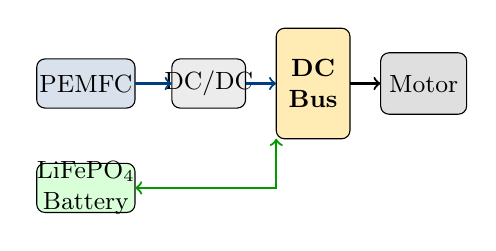
\begin{tikzpicture}[scale=0.78, font=\small]
          \draw[fill=fcblue!15, rounded corners=3pt] (0,2.0) rectangle (1.6,2.8) node[midway]{PEMFC};
          \draw[fill=gray!15, rounded corners=3pt] (2.2,2.0) rectangle (3.4,2.8) node[midway]{DC/DC};
          \draw[fill=fcgold!30, rounded corners=3pt] (3.9,1.5) rectangle (5.1,3.3) node[midway,align=center]{\textbf{DC}\\\textbf{Bus}};
          \draw[fill=green!15, rounded corners=3pt] (0,0.3) rectangle (1.6,1.1) node[midway,align=center]{LiFePO$_4$\\Battery};
          \draw[fill=gray!25, rounded corners=3pt] (5.6,1.9) rectangle (7.0,2.9) node[midway]{Motor};
          \draw[->, thick, fcblue] (1.6,2.4) -- (2.2,2.4);
          \draw[->, thick, fcblue] (3.4,2.4) -- (3.9,2.4);
          \draw[<->, thick, green!60!black] (1.6,0.7) -- (3.9,0.7) -- (3.9,1.5);
          \draw[->, thick] (5.1,2.4) -- (5.6,2.4);
        \end{tikzpicture}
      \end{block}
    \end{column}
    \begin{column}{0.45\textwidth}
      \begin{block}{Reference Vehicle: Toyota Mirai II}
        \begin{tabular}{@{}ll@{}}
          \toprule
          \textbf{Parameter} & \textbf{Value} \\
          \midrule
          Total mass & 1925 kg \\
          Frontal area & 2.547 m$^2$ \\
          Drag coeff.\ $C_D$ & 0.29 \\
          FC stack peak & 128 kW (gross) \\
          DC/DC efficiency & 0.95 \\
          Battery (rescaled) & $\approx$7.92 kWh \\
          \bottomrule
        \end{tabular}
      \end{block}
      \vspace{4pt}
      \begin{block}{Drive Cycle}
        \begin{itemize}
          \item $2\times$ WLTP Class 3b — total 1 h, 46.5 km
          \item Flat road ($\alpha=0$), $\Delta t = 1\,\text{s}$, $N=3600$ decisions
          \item Allows meaningful SoC depletion from 0.90 to 0.25
        \end{itemize}
      \end{block}
    \end{column}
  \end{columns}
\end{frame}
\note{
  We chose the T4 topology because the unidirectional DC/DC converter on the fuel cell side
  provides natural isolation and protects the stack from reverse current, while keeping the
  control problem tractable with a single decision variable. \\[4pt]
  The Toyota Mirai II was selected because it is the best-selling production fuel cell car with a
  complete and publicly available energy balance. We kept all vehicle parameters at their
  published values and only rescaled the battery to 7.92 kWh to enable the plug-in functionality. \\[4pt]
  The reference trip uses two consecutive WLTP Class 3b cycles — one hour and 46.5 km — which
  is sufficient to deplete the battery from 90\% to 25\% SoC.
}

% ============================================================
%  SLIDE 6 — PEMFC MODEL
% ============================================================
\begin{frame}{Mathematical Modeling (1/2): PEMFC — Mann–Amphlett GSSEM}
  \begin{columns}[T]
    \begin{column}{0.52\textwidth}
      \begin{block}{Cell Voltage Decomposition (Polarization Curve)}
        \[
          V_{\mathrm{cell}} = E_{\mathrm{Nernst}} - V_{\mathrm{act}} - V_{\mathrm{ohm}} - V_{\mathrm{con}}
        \]
        \begin{itemize}
          \item \textbf{Nernst potential} (thermodynamic limit):
          \[
            E_N = 1.229 - 8.5\!\times\!10^{-4}(T\!-\!298.15)
                  + 4.31\!\times\!10^{-5}T\!\ln\!\bigl(p^*_{H_2}\,p^{*1/2}_{O_2}\bigr)
          \]
          \item \textbf{Activation loss} (Tafel semi-empirical):
          \[
            V_{\mathrm{act}} = -\bigl[\xi_1 + \xi_2 T + \xi_3 T\ln C^*_{O_2} + \xi_4 T\ln i\bigr]
          \]
          \item \textbf{Ohmic loss}: $V_{\mathrm{ohm}} = i(R_m + R_c)$
          \item \textbf{Concentration loss}:
          $V_{\mathrm{con}} = -\beta\ln\!\bigl(1 - J/J_{\max}\bigr)$
        \end{itemize}
      \end{block}
    \end{column}
    \begin{column}{0.45\textwidth}
      \begin{block}{From Voltage to H$_2$ Consumption}
        Stack power and hydrogen flow rate:
        \[
          \dot{m}_{H_2} = \frac{P_{\mathrm{FC,gross}}}{\etaFC(P_{\mathrm{FC,gross}})\cdot\LHV}
        \]
        $\etaFC(\cdot)$ stored as a 1-D look-up table ($\approx 0.70$ at 12 kW, $\approx 0.54$ at max)
      \end{block}
      \vspace{4pt}
      \begin{alertblock}{Why a \emph{Static} (0-D) Model?}
        \begin{itemize}
          \item Dynamic models require ODE integration at \textbf{every DP grid point}
          \item Static (GSSEM): only algebraic evaluations
          \item \highlight{Reduces computational load by $>100\times$} vs.\ dynamic formulation
          \item Steady-state error: only a few \%; acceptable for EMS-level design
          \item Stack temperature regulated externally; EMS acts on $\sim$1 s timescale
        \end{itemize}
      \end{alertblock}
    \end{column}
  \end{columns}
\end{frame}
\note{
  The PEMFC model is central to the whole framework because it maps the control decision —
  stack power — to the hydrogen consumption cost. \\[4pt]
  The Mann–Amphlett GSSEM expresses the cell voltage as the Nernst thermodynamic potential
  minus three loss terms: activation, ohmic, and concentration. Each term has a clear physical
  interpretation. The activation loss dominates at low currents, the ohmic loss scales linearly
  with current, and the concentration loss blows up near the limiting current density. \\[4pt]
  The decisive reason for choosing this static model is computational. Dynamic 0-D models like
  that of Ziogou et al.\ require solving ODEs at every grid point of the DP algorithm.
  An operation-count analysis that I carried out showed that the static formulation reduces the
  computational load by more than two orders of magnitude, at the cost of a steady-state error
  of only a few per cent — which is entirely acceptable at the EMS design stage.
}

% ============================================================
%  SLIDE 7 — BATTERY MODEL
% ============================================================
\begin{frame}{Mathematical Modeling (2/2): Battery — 1-RC + Hysteresis}
  \begin{columns}[T]
    \begin{column}{0.52\textwidth}
      \begin{block}{Model Equations}
        \textbf{RC relaxation voltage} (discrete):
        \[
          V_{RC}(k\!+\!1) = a\,V_{RC}(k) + b\,i_b, \quad
          a = e^{-\Delta t/\tau_1},\; b = R_1(1-a)
        \]
        \textbf{Coulomb counting} (SoC state equation):
        \[
          \SoC(k\!+\!1) = \SoC(k) - \frac{\eta_c\,\Delta t}{Q_{\mathrm{pack}}}\,i_b
        \]
        \textbf{Terminal voltage}:
        \[
          V_b = V_{OC}(\SoC,\,\mathrm{dir}) - i_b R_s - V_{RC}
        \]
        \textbf{Hysteresis OCV law} (Huria et al.):
        \[
          \frac{dV_{OC}}{d\SoC} = \frac{dV_{OC}^{\mathrm{ref}}}{d\SoC}
                                  + \gamma_h(V_{OC}^{\mathrm{ref}} - V_{OC})
        \]
      \end{block}
    \end{column}
    \begin{column}{0.45\textwidth}
      \begin{alertblock}{Why 1-RC + Hysteresis for LiFePO$_4$?}
        \begin{center}
          \textit{[Figure 1 — OCV–SoC curve of LiFePO$_4$]}
        \end{center}
        \vspace{4pt}
        \begin{itemize}
          \item LFP OCV curve is \highlight{nearly flat} between 20\%–80\% SoC
          \item A simple $R_{\mathrm{int}}$ model cannot distinguish charge from discharge states at the same SoC
          \item Hysteresis state tracks the \textbf{direction-dependent} OCV branches
          \item Nejad et al.: 1-RC+Hys achieves \highlight{1.39\% mean SoC error} — lowest among 10 ECMs
        \end{itemize}
        \vspace{4pt}
        Pack: 96s10p, $A123$ ANR26650M1B ($\mathrm{LiFePO_4}$),\\
        $Q_{\mathrm{pack}} = 25\,\text{Ah}$, $V_{\mathrm{nom}} = 316.8\,\text{V}$,\\
        $E_{\mathrm{nom}} = 7.92\,\text{kWh}$
      \end{alertblock}
    \end{column}
  \end{columns}
\end{frame}
\note{
  The battery model choice was driven by the chemistry. LiFePO4 has an almost flat
  open-circuit-voltage curve between 20 and 80\% SoC. This means that a simple internal
  resistance model that maps OCV to SoC with a single lookup cannot tell whether the cell
  is at 40\% SoC on a charge sweep or a discharge sweep — the OCV is nearly identical. \\[4pt]
  The hysteresis state solves this by tracking two direction-dependent OCV branches — a charge
  branch and a discharge branch — and interpolating between them according to the law of
  Huria et al. \\[4pt]
  We also follow a two-level modeling approach: the full 1-RC + Hysteresis model is used for
  physical simulation (the plant), while the EMS optimization layer uses the simpler Rint model
  to keep the online computation tractable.
}

% ============================================================
%  SLIDE 8 — COST FUNCTION
% ============================================================
\begin{frame}{Power Flow Model \& Cost Function}
  \begin{columns}[T]
    \begin{column}{0.52\textwidth}
      \begin{block}{Per-Step Running Cost}
        \textbf{Hydrogen cost} (FC side):
        \[
          C_{\mathrm{FC},k} = \MH \cdot
            \frac{P_{\mathrm{FC,bus},k}/\eta_{dc} + P_{\mathrm{aux},k}}
                 {\etaFC(\cdot)\cdot\LHV}\,\Delta t
        \]
        \textbf{Electricity cost} (battery side):
        \[
          C_{\mathrm{bat},k} = \Mel' \cdot
            \frac{P_{\mathrm{bat},k}}{\eta_{\mathrm{eff}}(P_{\mathrm{bat},k},\SoC_k)}\,\Delta t
        \]
        Direction-dependent round-trip efficiency:
        \[
          \eta_{\mathrm{eff}}(P_{\mathrm{bat}}) =
            (\eta_{\mathrm{chg}}\,\eta_{\mathrm{dis}})^{\operatorname{sgn}(P_{\mathrm{bat}})}
        \]
        \textbf{Total cost functional}:
        \[
          \boxed{J = \sum_{k=0}^{N-1}\!\bigl(C_{\mathrm{FC},k}+C_{\mathrm{bat},k}\bigr)
                    + \underbrace{\gamma(\SoC_N - \SoC_{\mathrm{target}})^2}_{\text{terminal penalty}}}
        \]
      \end{block}
    \end{column}
    \begin{column}{0.45\textwidth}
      \begin{block}{Germany 2026 Price Scenarios}
        \renewcommand{\arraystretch}{1.3}
        \begin{tabular}{@{}lccc@{}}
          \toprule
          Scenario & $\MH$ & $\Mel$ & \\
          & (€/kg) & (€/kWh) & \\
          \midrule
          High   & 13.85 & 0.40 & \\
          \highlight{Default} & \highlight{11.00} & \highlight{0.35} & \highlight{$\star$} \\
          Low    & 8.00  & 0.32 & \\
          \bottomrule
        \end{tabular}
      \end{block}
      \vspace{6pt}
      \begin{alertblock}{Key Insight}
        In the \textit{default} scenario, grid electricity is cheaper than hydrogen
        on a lower-heating-value basis
        \[
          \frac{\Mel}{\eta_{\mathrm{eff}}} \ll \frac{\MH}{\etaFC\cdot\LHV}
        \]
        $\Rightarrow$ Optimal strategy: \highlight{maximize battery usage} within constraints.\\[4pt]
        Penalty weight: $\gamma = 1000\,\text{€}$ (1 unit SoC error $\gg$ trip cost of 5–15 €)
      \end{alertblock}
    \end{column}
  \end{columns}
\end{frame}
\note{
  The cost function is the principal mathematical result of MAT 4901E. It combines two monetary
  flows: hydrogen cost and electricity cost. \\[4pt]
  The hydrogen cost per step is straightforward: multiply the hydrogen mass flow by the price.
  The electricity cost is more subtle because we have to account for direction-dependent
  round-trip losses. When the battery discharges, we must account for the extra grid energy that
  was originally invested; when it charges via regenerative braking, we credit only the
  recoverable fraction. This prevents the optimizer from treating charging and discharging
  symmetrically, which would be physically incorrect. \\[4pt]
  The terminal soft penalty with gamma = 1000 euros ensures the battery reaches the 25\% SoC
  target without making the optimization infeasible. The scaling is chosen so that a 1\% SoC
  deviation costs roughly the same as the entire trip cost. \\[4pt]
  In the default Germany 2026 scenario, electricity at 0.35 €/kWh is much cheaper than
  hydrogen at 11 €/kg on an energy basis, so we theoretically expect the optimal strategy to
  deplete the battery as much as possible before using the fuel cell.
}

% ============================================================
%  SLIDE 9 — CONTROL STRATEGIES OVERVIEW
% ============================================================
\begin{frame}{Energy Management Strategies — Overview}
  \begin{block}{Four Candidate Strategies (to be compared in MAT 4902E)}
  \renewcommand{\arraystretch}{1.35}
  \resizebox{\textwidth}{!}{%
  \begin{tabular}{@{}lcccc@{}}
    \toprule
    \textbf{Property} & \textbf{DP} & \textbf{A-ECMS} & \textbf{MPC} & \textbf{BLFS} \\
    \midrule
    Mathematical basis & Bellman recursion & Pontryagin PMP & Finite-horizon OCP & Hysteresis rule \\
    Information required & Full cycle (offline) & Instantaneous + SoC ref. & Finite horizon ($N_p$) & Instantaneous SoC \\
    Optimality & \highlight{Global optimum} & Near-optimal (PMP) & Local optimum & None (rule-based) \\
    Real-time capable & \textcolor{red}{\textbf{No}} & \textcolor{green!60!black}{\textbf{Yes}} & \textcolor{green!60!black}{\textbf{Yes}} & \textcolor{green!60!black}{\textbf{Yes}} \\
    Computational load & High (offline) & Low & Medium & Very low \\
    Role in study & \textbf{Benchmark} & Production candidate & Production candidate & Protection layer \\
    \bottomrule
  \end{tabular}}
  \end{block}
  \vspace{4pt}
  \begin{columns}
    \begin{column}{0.48\textwidth}
      \begin{block}{DP Bellman Recursion (Benchmark)}
        \[
          V_k(\SoC_k) = \min_{u_k}\bigl\{L_k(\SoC_k, u_k) + V_{k+1}(\SoC_{k+1})\bigr\}
        \]
        Grid: $\Delta\SoC = 0.005$, $\Delta\PFC = 1\,\text{kW}$
      \end{block}
    \end{column}
    \begin{column}{0.48\textwidth}
      \begin{block}{A-ECMS: PI-Adapted Equivalence Factor}
        \[
          H = L(\SoC,\PFC) + \lambda\,\dot{\SoC}
        \]
        \[
          s(t) = s_0 + m\,e_{\SoC}(t) + n\!\int_0^t\!e_{\SoC}\,d\tau
        \]
      \end{block}
    \end{column}
  \end{columns}
\end{frame}
\note{
  We formulated four strategies, each at a different point on the optimality-vs-implementability
  spectrum. \\[4pt]
  Dynamic Programming is the gold standard: it finds the mathematically global optimum by
  backward recursion over the Bellman equation. However, it requires knowledge of the entire
  drive cycle in advance and is computationally heavy, so it can only be used offline as a
  benchmark. \\[4pt]
  Adaptive ECMS is the real-time counterpart of DP. It is grounded in Pontryagin's Minimum
  Principle, which says the optimal decision minimizes the Hamiltonian at every instant. The
  equivalence factor — which converts battery energy to a fuel equivalent — is adapted online
  via a PI controller that tracks a linear SoC reference trajectory. This is critical in the plug-in
  case: a constant equivalence factor can push the strategy to degenerate into pure
  charge-depleting or charge-sustaining behavior. \\[4pt]
  MPC solves the same optimization problem but only over a short prediction horizon of 15 steps,
  applying only the first control action and re-solving at every instant. \\[4pt]
  BLFS is not an independent strategy — it is a protection layer that runs under A-ECMS or MPC.
  It enforces a hysteresis band around the SoC reference and limits the fuel cell ramp rate to
  5 kW/s to prevent membrane stress.
}

% ============================================================
%  SLIDE 10 — STRATEGIES DETAIL
% ============================================================
\begin{frame}{Energy Management Strategies — Formulations}
  \begin{columns}[T]
    \begin{column}{0.48\textwidth}
      \begin{block}{MPC — Receding Horizon ($N_p = 15$)}
        At each step $k$, solve:
        \[
          \min_{\{\PFC\}_{j=k}^{k+N_p-1}}\;
          \sum_{j=k}^{k+N_p-1} L_j + \gamma_{\mathrm{MPC}}\,e_{\SoC,k+N_p}^2
        \]
        Subject to dynamics (Eq.\ 18) and limits (Eq.\ 26). \\
        Apply only $\PFC(k)$; repeat at $k+1$. \\
        Assumes \textbf{constant future load} over horizon.
      \end{block}
      \vspace{4pt}
      \begin{block}{Current Status (MAT 4901E)}
        \begin{itemize}
          \item[$\checkmark$] Literature review complete
          \item[$\checkmark$] All architectural selections fixed
          \item[$\checkmark$] All component models formulated
          \item[$\checkmark$] Cost functional derived (Eq.\ 24)
          \item[$\checkmark$] Complete OCP stated (Eqs.\ 25–26)
          \item[$\checkmark$] All four strategies formulated
        \end{itemize}
      \end{block}
    \end{column}
    \begin{column}{0.48\textwidth}
      \begin{block}{BLFS — Boundary Layer Protection}
        Define SoC error band $[\SoC_{\mathrm{ref}}\pm\delta]$, $\delta=0.05$:
        \[
          \PFC(t) = \begin{cases}
            \PFC^{\min} & \SoC > \SoC_{\mathrm{ref}} + \delta \\
            \PFC^{\star} & |\SoC - \SoC_{\mathrm{ref}}| \le \delta \\
            \PFC^{\mathrm{eff}} & \SoC < \SoC_{\mathrm{ref}} - \delta
          \end{cases}
        \]
        \vspace{2pt}
        Fuel cell ramp-rate limit:
        \[
          \left|\frac{d\PFC}{dt}\right| \le 5\;\text{kW/s}
        \]
        $\Rightarrow$ Prevents gas starvation \& membrane fatigue
      \end{block}
      \vspace{4pt}
      \begin{alertblock}{Comparison Metrics (MAT 4902E)}
        Total cost (€/100 km), $H_2$ \& electricity consumed, terminal SoC accuracy, FC quasi-stability, per-step computation time
      \end{alertblock}
    \end{column}
  \end{columns}
\end{frame}
\note{
  Here I present the two remaining strategies in more detail. \\[4pt]
  The MPC formulation is essentially a finite-horizon version of the DP problem. At every
  sampling instant we solve a short optimization over the next 15 seconds, assuming the
  future load is constant at the current value, apply only the first control action, and
  repeat. This makes MPC causal and implementable in real time, but it cannot achieve the
  global optimum because it has limited look-ahead. \\[4pt]
  BLFS is a rule-based protection layer. It defines a hysteresis band of ±5\% SoC around the
  reference trajectory. Outside the band, the fuel cell is forced to a fixed operating point
  (minimum or peak-efficiency power); inside the band, the upper-level strategy's command
  passes through. The ramp-rate limit of 5 kW/s is a physical constraint that prevents
  hydrogen starvation and membrane fatigue — it appears in the control law but not in the
  monetary cost functional. \\[4pt]
  In MAT 4902E we will compare all four strategies against each other on the five metrics
  listed here.
}

% ============================================================
%  SLIDE 11 — FUTURE WORK
% ============================================================
\begin{frame}{Future Work: MAT 4902E Road Map}
  \begin{columns}[T]
    \begin{column}{0.52\textwidth}
      \begin{block}{\faIcon{python}\; Step 1 — Two-Layer Simulation in Python}
        \begin{itemize}
          \item \textbf{Plant layer}: Mann–Amphlett stack + full 1-RC+Hysteresis battery
          \item \textbf{Controller layer}: efficiency LUT + Rint model (fast)
          \item WLTP drive cycle playback at $\Delta t = 1\,\text{s}$
        \end{itemize}
      \end{block}
      \vspace{6pt}
      \begin{block}{\faIcon{search}\; Step 2 — Metaheuristic Parameter Identification}
        \begin{itemize}
          \item Identify GSSEM coefficients $\{\xi_1,\xi_2,\xi_3,\xi_4,\beta\}$ for the \textbf{Mirai II stack} from published polarization data
          \item Algorithms: \highlight{PSO} (Particle Swarm Optimization) and \highlight{GA} (Genetic Algorithm)
          \item Generate the efficiency map $\etaFC(P_{\mathrm{FC}})$ as a 1-D LUT
        \end{itemize}
      \end{block}
    \end{column}
    \begin{column}{0.45\textwidth}
      \begin{block}{\faIcon{chart-bar}\; Step 3 — Strategy Implementation \& Comparison}
        \begin{enumerate}
          \item DP by backward Bellman recursion (benchmark)
          \item A-ECMS with PI-adapted equivalence factor
          \item MPC transcribed as QP, solved at each step
          \item BLFS layer integrated under A-ECMS / MPC
        \end{enumerate}
      \end{block}
      \vspace{4pt}
      \begin{alertblock}{\faIcon{trophy}\; Expected Outcome}
        A quantitative ranking of the four strategies on:
        \[
          \text{Total cost} \;\left[\frac{\text{€}}{100\,\text{km}}\right],\;
          \dot{m}_{H_2},\; \Delta\SoC_{\mathrm{terminal}}
        \]
        plus a price-scenario sensitivity analysis (Table 3).
      \end{alertblock}
    \end{column}
  \end{columns}
\end{frame}
\note{
  In MAT 4902E — next semester — the work will shift from formulation to numerical solution
  and comparison. \\[4pt]
  The first task is to build a two-layer simulation environment in Python. The plant layer
  uses all the high-fidelity models we derived this semester; the controller layer uses simplified
  models to keep the optimization tractable. \\[4pt]
  The second task is to identify the GSSEM coefficients for the actual Toyota Mirai II stack.
  The published polarization data gives us measured current-voltage points; we will fit the
  five semi-empirical coefficients using Particle Swarm Optimization and Genetic Algorithms.
  This produces the efficiency map that all four strategies will use. \\[4pt]
  The third task is to implement and compare all four strategies. DP gives the global optimum
  as a benchmark. A-ECMS, MPC, and BLFS are the real-time candidates. We will report the
  total operating cost in euros per 100 km, hydrogen and electricity consumption, terminal
  SoC accuracy, fuel cell ramp stability, and per-step computation time. A sensitivity analysis
  over the three Germany 2026 price scenarios will show how robust each strategy is to
  market conditions.
}

% ============================================================
%  SLIDE 12 — THANK YOU / Q&A
% ============================================================
\begin{frame}{Summary \& Conclusions}
  \begin{columns}[T]
    \begin{column}{0.5\textwidth}
      \begin{block}{What Was Achieved in MAT 4901E}
        \begin{enumerate}
          \item[$\checkmark$] Comprehensive literature review (EMS, PEMFC, Li-ion)
          \item[$\checkmark$] T4 topology \& Toyota Mirai II selected \& justified
          \item[$\checkmark$] PEMFC modeled via Mann–Amphlett GSSEM
          \item[$\checkmark$] Battery modeled via 1-RC + Hysteresis (LiFePO$_4$)
          \item[$\checkmark$] Plug-in monetary cost function derived
          \item[$\checkmark$] Complete OCP stated (Eqs.\ 25–26)
          \item[$\checkmark$] Four EMS strategies formulated (DP, A-ECMS, MPC, BLFS)
        \end{enumerate}
      \end{block}
    \end{column}
    \begin{column}{0.47\textwidth}
      \begin{alertblock}{The Central Result}
        \[
          J = \sum_{k=0}^{N-1}\!\bigl[C_{\mathrm{FC},k}(u_k) + C_{\mathrm{bat},k}(x_k,u_k)\bigr]
              + \gamma\bigl(\SoC_N - \SoC_{\mathrm{tgt}}\bigr)^2
        \]
        A rigorous, Europe-calibrated monetary cost functional for plug-in FCHEV optimization — ready for numerical solution.
      \end{alertblock}
      \vspace{8pt}
      \begin{center}
        \large\textbf{Thank you for your attention.}\\[8pt]
        \normalsize Questions are welcome.
      \end{center}
    \end{column}
  \end{columns}
\end{frame}
\note{
  To summarize: in MAT 4901E we completed the full mathematical foundation of the project.
  We have a physically accurate PEMFC model, a chemically appropriate battery model,
  a monetary cost function calibrated to Germany 2026 prices, and four rigorously formulated
  control strategies. \\[4pt]
  The central result is the cost functional in the box — it is the principal mathematical
  contribution of this semester and the starting point for all numerical work in MAT 4902E. \\[4pt]
  Thank you, and I am happy to take questions.
}

\end{document}
